

% ─────────────────────────────────────────────────────────────────────────────
% TABLE A: Full candidate matrix — WITH deterministic trend (Appendix)
% ─────────────────────────────────────────────────────────────────────────────

\begin{table}[H]
	\centering
	\footnotesize
	\caption{ARDL(2,4) Coefficient Comparison — With Deterministic Trend
		(\textit{Appendix})}
	\label{tab:S0_candidates_trend}
	\begin{threeparttable}
		\adjustbox{max width=\linewidth}{%
			\begin{tabular}{lrrrrr}
				\toprule\toprule
				& Shaikh (2016)
				& C1 $(K^G,\, p^{IG})$
				& C2 $(K^{TC},\, p^{IG})$
				& C3 $(K^G,\, p^{KN})$
				& C4 $(K^{TC},\, p^{KN})$ \\
				\hline\hline
				%
				% ── Short-run coefficients ──────────────────────────────────────────
				%
				\multicolumn{6}{l}{\textit{Panel A: Short-run coefficients}} \\[2pt]
				%
				$L_1 y_t$
				&  1.298  &  0.811  &  0.745  &  1.240  &  0.996  \\
				$L_2 y_t$
				& $-$0.393  & $-$0.003  &  0.062  & $-$0.325  & $-$0.105  \\[4pt]
				%
				$k_t$ (L0)
				&  5.086  &  1.267  &  1.270  &  4.325  &  2.110  \\
				$L_1 k_t$
				& $-$14.285  & $-$1.192  & $-$1.087  & $-$11.700  & $-$2.947  \\
				$L_2 k_t$
				&  15.705  & $-$0.381  & $-$0.428  &  12.300  &  0.345  \\
				$L_3 k_t$
				& $-$8.296  &  0.146  &  0.111  & $-$6.262  &  0.777  \\
				$L_4 k_t$
				&  1.853  &  0.091  &  0.036  &  1.415  & $-$0.196  \\[4pt]
				%
				$d_{1956}$
				& $-$0.071  & $-$0.035  & $-$0.035  & $-$0.062  & $-$0.052  \\
				$d_{1974}$
				& $-$0.081  & $-$0.129  & $-$0.125  & $-$0.082  & $-$0.100  \\
				$d_{1980}$
				& $-$0.045  & $-$0.065  & $-$0.058  & $-$0.044  & $-$0.047  \\[4pt]
				%
				Constant
				&  0.207  &  0.400  &  0.456  &  0.005  &  0.009  \\
				Trend
				& ---  &  0.013  &  0.014  & $-$0.001  & $-$0.000  \\[4pt]
				%
				% ── Long-run multipliers ────────────────────────────────────────────
				%
				\midrule
				\multicolumn{6}{l}{\textit{Panel B: Long-run multipliers}} \\[2pt]
				%
				$1 - \Sigma\gamma$
				&  0.095  &  0.192  &  0.193  &  0.085  &  0.110  \\
				$\hat{\theta}$
				&  0.661  & $-$0.358  & $-$0.510  &  0.955  &  0.815  \\
				$\hat{a}$ (intercept)
				&  2.178  &  2.082  &  2.365  &  0.063  &  0.084  \\[4pt]
				$d_{1956}$ (LR)
				& $-$0.743  & $-$0.182  & $-$0.181  & $-$0.730  & $-$0.472  \\
				$d_{1974}$ (LR)
				& $-$0.855  & $-$0.672  & $-$0.649  & $-$0.970  & $-$0.906  \\
				$d_{1980}$ (LR)
				& $-$0.478  & $-$0.337  & $-$0.298  & $-$0.518  & $-$0.427  \\[4pt]
				%
				% ── Fit statistics ──────────────────────────────────────────────────
				%
				\midrule
				\multicolumn{6}{l}{\textit{Panel C: Fit statistics}} \\[2pt]
				%
				$R^2$
				&  0.9992  &  0.9993  &  0.9995  &  0.9993  &  0.9987  \\
				Adj.\ $R^2$
				&  0.9990  &  0.9992  &  0.9994  &  0.9991  &  0.9985  \\
				RMSE
				&  0.016  &  0.023  &  0.021  &  0.017  &  0.022  \\
				%
				\bottomrule
		\end{tabular}}
		\begin{tablenotes}
			\item \textit{Notes:}
			$y_t \equiv \ln(\text{GVAcorp}_t / p_t)$ and
			$k_t \equiv \ln(K^G_t / p_t)$ for columns C1 and C3;
			$k_t \equiv \ln(K^{TC}_t / p_t)$ for columns C2 and C4.
			$K^G$ is the gross corporate capital stock reconstructed via
			Shaikh's Generalized Perpetual Inventory Method (GPIM);
			see Appendix~\ref{app:gpim} for derivation.
			$K^{TC} = K^G + \text{Inventories}$.
			$p^{IG}$ is the implicit price deflator of corporate gross investment
			($p^{IG} \equiv \text{IGCcorp}/\text{IGRcorp} \times 100$,
			Fixed Assets Table~6.7/6.8).
			$p^{KN}$ is the implicit price deflator of Shaikh's GPIM-adjusted
			net corporate capital stock
			($p^{KN} \equiv \text{KNCcorp}/\text{KNRcorp} \times 100$,
			Appendix Table~6.8.II.1).
			Step dummies $d_{1956}$, $d_{1974}$, $d_{1980}$ are impulse dummies
			(equal to 1 in the break year only);
			long-run effects computed as $\hat{c}_h/(1-\Sigma\hat{\gamma}_i)$.
			Sample: 1951--2011 ($N=61$).
		\end{tablenotes}
	\end{threeparttable}
\end{table}


% ─────────────────────────────────────────────────────────────────────────────
% TABLE B: Full candidate matrix — WITHOUT deterministic trend (Appendix)
% ─────────────────────────────────────────────────────────────────────────────
\pagebreak
\begin{table}[H]
	\centering
    \footnotesize
	\caption{ARDL(2,4) Coefficient Comparison --- Without Deterministic Trend
		(\textit{Appendix})}
	\label{tab:S0_candidates_notrend}
	\begin{threeparttable}
		\adjustbox{max width=\linewidth}{%
			\begin{tabular}{lrrrrr}
				\toprule\toprule
				& Shaikh (2016)
				& C1 $(K^G,\, p^{IG})$
				& C2 $(K^{TC},\, p^{IG})$
				& \textbf{C3} $\bm{(K^G,\, p^{KN})}$
				& C4 $(K^{TC},\, p^{KN})$ \\
				\hline\hline
				%
				% ── Short-run coefficients ──────────────────────────────────────────
				%
				\multicolumn{6}{l}{\textit{Panel A: Short-run coefficients}} \\[2pt]
				%
				$L_1 y_t$
				&  1.298  &  0.903  &  0.874  &  \textbf{1.242}  &  0.995  \\
				$L_2 y_t$
				& $-$0.393  & $-$0.038  & $-$0.006  & $\bm{-}$\textbf{0.338}  & $-$0.109  \\[4pt]
				%
				$k_t$ (L0)
				&  5.086  &  1.344  &  1.321  &  \textbf{4.378}  &  2.122  \\
				$L_1 k_t$
				& $-$14.285  & $-$1.291  & $-$1.193  & $\bm{-}$\textbf{11.754}  & $-$2.948  \\
				$L_2 k_t$
				&  15.705  & $-$0.333  & $-$0.335  &  \textbf{12.386}  &  0.353  \\
				$L_3 k_t$
				& $-$8.296  &  0.206  &  0.180  & $\bm{-}$\textbf{6.350}  &  0.770  \\
				$L_4 k_t$
				&  1.853  &  0.183  &  0.135  &  \textbf{1.409}  & $-$0.210  \\[4pt]
				%
				$d_{1956}$
				& $-$0.071  & $-$0.045  & $-$0.045  & $\bm{-}$\textbf{0.062}  & $-$0.052  \\
				$d_{1974}$
				& $-$0.081  & $-$0.137  & $-$0.134  & $\bm{-}$\textbf{0.081}  & $-$0.099  \\
				$d_{1980}$
				& $-$0.045  & $-$0.067  & $-$0.060  & $\bm{-}$\textbf{0.044}  & $-$0.047  \\[4pt]
				%
				Constant
				&  0.207  &  0.013  & $-$0.015  &  \textbf{0.055}  &  0.024  \\[4pt]
				%
				% ── Long-run multipliers ────────────────────────────────────────────
				%
				\midrule
				\multicolumn{6}{l}{\textit{Panel B: Long-run multipliers}} \\[2pt]
				%
				$1 - \Sigma\gamma$
				&  0.095  &  0.135  &  0.132  &  \textbf{0.096}$^{\dagger}$  &  0.114  \\
				$\hat{\theta}$
				&  0.661  &  0.813  &  0.822  &  \textbf{0.720}  &  0.761  \\
				$\hat{a}$ (intercept)
				&  2.178  &  0.100  & $-$0.111  &  \textbf{0.570}  &  0.208  \\[4pt]
				$d_{1956}$ (LR)
				& $-$0.743  & $-$0.336  & $-$0.344  & $\bm{-}$\textbf{0.649}  & $-$0.454  \\
				$d_{1974}$ (LR)
				& $-$0.855  & $-$1.015  & $-$1.015  & $\bm{-}$\textbf{0.841}  & $-$0.869  \\
				$d_{1980}$ (LR)
				& $-$0.478  & $-$0.494  & $-$0.454  & $\bm{-}$\textbf{0.456}  & $-$0.410  \\[4pt]
				%
				% ── Fit statistics ──────────────────────────────────────────────────
				%
				\midrule
				\multicolumn{6}{l}{\textit{Panel C: Fit statistics}} \\[2pt]
				%
				$R^2$
				&  0.9992  &  0.9993  &  0.9994  &  \textbf{0.9993}  &  0.9987  \\
				Adj.\ $R^2$
				&  0.9990  &  0.9991  &  0.9993  &  \textbf{0.9991}  &  0.9985  \\
				RMSE
				&  0.016  &  0.024  &  0.022  &  \textbf{0.017}$^{\dagger}$  &  0.022  \\
				%
				\bottomrule
		\end{tabular}}
		\begin{tablenotes}
			\item \textit{Notes:}
			$y_t \equiv \ln(\text{GVAcorp}_t / p_t)$ and
			$k_t \equiv \ln(K^G_t / p_t)$ for columns C1 and C3;
			$k_t \equiv \ln(K^{TC}_t / p_t)$ for columns C2 and C4.
			$K^G$ is the gross corporate capital stock reconstructed via Shaikh's GPIM;
			$K^{TC} = K^G + \text{Inventories}$.
			$p^{IG}$: implicit deflator of corporate gross investment.
			$p^{KN}$: implicit deflator of GPIM-adjusted net corporate stock
			($p^{KN} \equiv \text{KNCcorp}/\text{KNRcorp} \times 100$).
			Step dummies are impulse dummies (value 1 in break year only).
			Boldface: preferred specification C3 $(K^G, p^{KN})$.
			$^{\dagger}$ Matches Shaikh's published target within rounding
			(target: $1 - \Sigma\gamma = 0.095$; RMSE $= 0.016$).
			Sample: 1951--2011 ($N=61$).
		\end{tablenotes}
	\end{threeparttable}
\end{table}

% =============================================================================
% APPENDIX: S1 Extended Figures
% Place inside \section{Critical Replication Extended Results}
% \label{app:critical_replication_results_extended}
% =============================================================================

\subsection{S1: ARDL Specification Geometry --- Extended Figures}
\label{app:S1_geometry}

\begin{figure}[htbp]
	\centering
	
\includegraphics[width=\textwidth]{figures/fig_S1_global_frontier.pdf}
	\caption{Pareto frontier of the admissible ARDL specification grid.
		Each point is an admissible specification in $\mathcal{A}_{S1}$
		($n = 65$), kernel-weighted by distance from the frontier
		(orange intensity decays exponentially with vertical distance).
		The dark envelope connects the specification with the lowest
		$-2\log L$ at each parameter count $k$, tracing the Pareto
		frontier from ARDL(1,2,$c_2$,$s_0$) at $k=5$ through the
		elbow at $k=9$--$11$ to the flat tail at $k \geq 12$.
		Envelope nodes are labeled $(p, q, c, s)$.
		The blue asterisk marks Shaikh's $m_0 = (2,4,c_3,s_3)$,
		inadmissible under proper PSS case discipline.
		Grey rug marks: marginal distribution of admissible specs
		by $-2\log L$ (left axis) and $k$ (bottom axis).
		See \S\ref{subsubsec:S1} for discussion.}
	\label{fig:S1_global_frontier}
\end{figure}

\pagebreak

\begin{figure}[htbp]
	\centering
	
\includegraphics[width=\textwidth]{figures/fig_S1_informational_domain.pdf}
	\caption{Informational domain $\mathcal{F}^{(0.20)}$ within the
		admissible specification grid.
		Orange points mark the 14 specifications in
		$\mathcal{F}^{(0.20)}$, defined as the bottom $20\%$ of
		$\mathcal{A}_{S1}$ by $-2\log L$ alone (no complexity
		penalty). Background kernel fading as in
		Figure~\ref{fig:S1_global_frontier}.
		Across $\mathcal{F}^{(0.20)}$, $\hat{\theta}$ ranges from
		$0.836$ to $0.864$ (mean $= 0.855$, sd $= 0.007$),
		confirming stability of the capacity anchor within the
		low-fit region of the admissible grid.
		The blue asterisk marks Shaikh's $m_0 = (2,4,c_3,s_3)$:
		inadmissible by the PSS bounds gate, yet inside
		$\mathcal{F}^{(0.20)}$ by fit, confirming that IC fitness
		and cointegration admissibility are independent filters.
		See \S\ref{subsubsec:S1} for discussion.}
	\label{fig:S1_informational_domain}
\end{figure}



% ============================================================
% Appendix: S2 Focal Diagnostics
% Place inside \section{} or \subsection{} for S2 diagnostics
% ============================================================

\subsection{S2 Focal Specification Diagnostics}
\label{app:S2_diagnostics}

\begin{figure}[!ht]
	\centering
	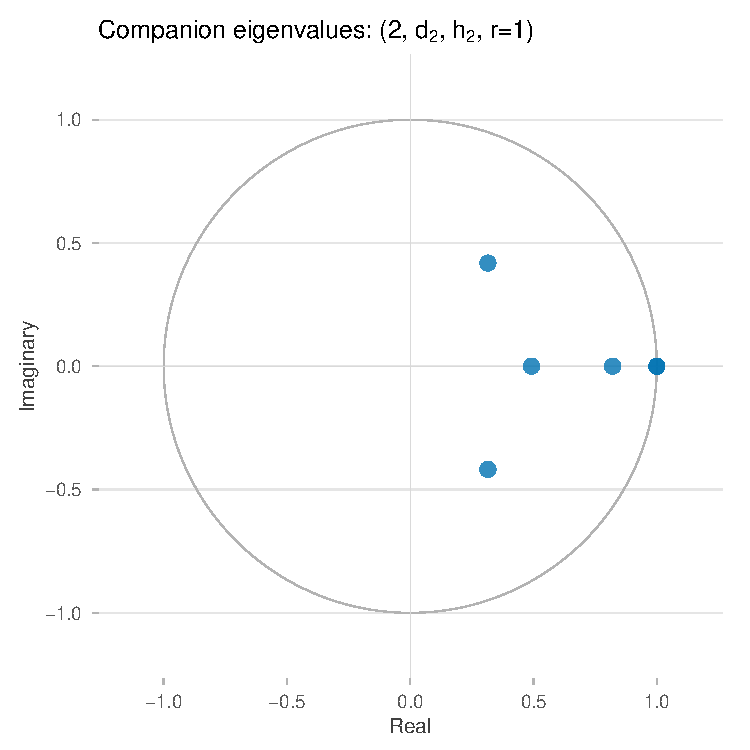
\includegraphics[width=0.7\textwidth]{figures/fig_S2_focal_companion.pdf}
	\caption{Companion matrix eigenvalues, focal specification
		$(p{=}2,\, d_2,\, h_2,\, r{=}1)$}
	\label{fig:S2_companion}
	
	\par\footnotesize\textit{Note:}
	Eigenvalue moduli of the companion matrix. The unit circle is shown
	for reference. Two eigenvalues sit on the unit circle, confirming
	exactly $m - r = 2$ common stochastic trends. All remaining roots
	lie strictly inside, confirming dynamic stability.
	Source: Dataset~1 (1947--2011); script~27.
\end{figure}

\begin{figure}[!ht]
	\centering
	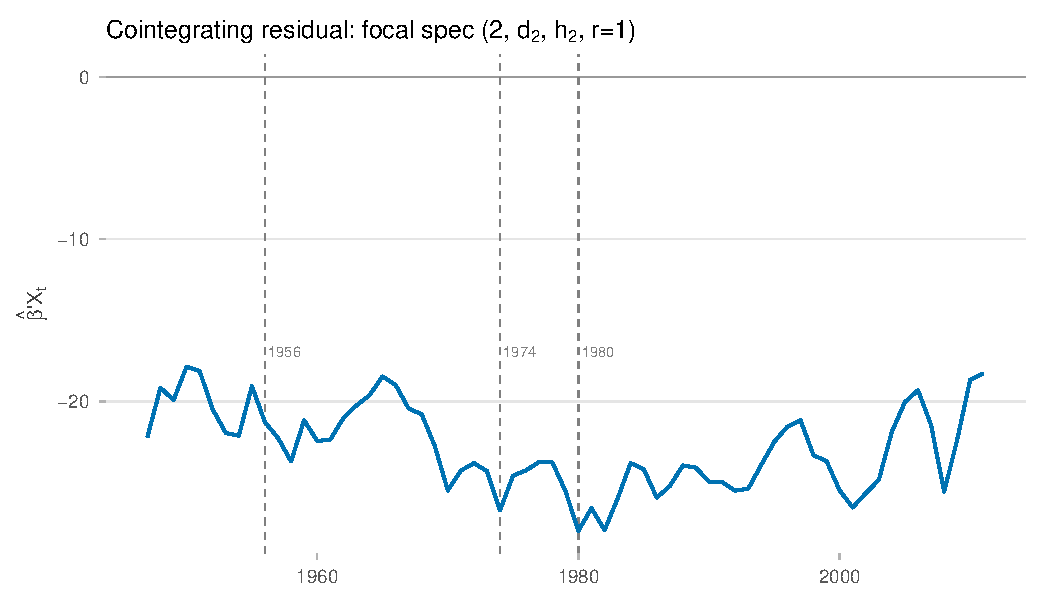
\includegraphics[width=\textwidth]{figures/fig_S2_focal_cu_path.pdf}
	\caption{Cointegrating residual $\hat{\beta}' X_t$, focal specification
		$(p{=}2,\, d_2,\, h_2,\, r{=}1)$}
	\label{fig:S2_focal_residual}
	
	\par\footnotesize\textit{Note:}
	This is the raw cointegrating residual
	$\hat{\beta}' X_t = \ln Y_t - 0.727\,\ln K_t + 20.022\,\ln e_t$,
	not the capacity utilization measure. The residual fluctuates around
	$-22.8$ because the large positive loading on $\ln e_t$ (whose values
	are negative throughout the sample) produces a persistent negative
	level; the mean is absorbed by the $d_2$ deterministic structure.
	The structural objects derived from this residual --- the capacity
	utilization path $\hat{u}_t$ and the reserve-army
	relation~(\ref{eq:S2_reserve_army}) --- are presented in
	Figures~\ref{fig:S2_focal_cu_exploitation}
	and~\ref{fig:S2_focal_scatter}.
	Vertical dashed lines mark the $h_2$ break dates (1956, 1974, 1980).
	Source: Dataset~1 (1947--2011); script~27.
\end{figure}